%% Full length research paper template
%% Created by Simon Hengchen and Nilo Pedrazzini for the Journal of Open Humanities Data (https://openhumanitiesdata.metajnl.com)

\documentclass{article}
\usepackage[english]{babel}
\usepackage[utf8]{inputenc}
\usepackage{johd}
\usepackage{hyperref}
\usepackage{longtable}

\title{Article Title Generation Using Recurrent Neural Networks With Attention}

\author{Dominik Matić$^{1}$$^{*}$\\
        C. L. F. Nimbus$^{2}$\\
        %\small $^{a}$Department, University, City, Country \\
        \small $^{1}$Faculty of Electrical Engineering and Computing, Zagreb, Croatia \\
        \small $^{2}$Šibenik, Croatia \\\\
        \small $^{*}$Corresponding author: Dominik Matić; \tt{dominik.matic@outlook.com}
}

\date{} %leave blank

\begin{document}

\maketitle

\begin{abstract} 
\noindent Recurrent neural networks, usually supported by attention mechanisms, can reliably solve many different problems such as text summarization and language translation. This paper experiments with limits of such networks by introducing a new type of problem: generating a title for an article given the abstract. This problem was chosen because it is similar enough to an already well-studied problem of text summarization, and also distinctly different from it in the fact that article titles don't necessarily have to be descriptive of the article in an obvious way. The scope of this paper includes an overview of related models and techniques used on similar problems, descriptions of how data was acquired and prepared, how the model was implemented and trained as well as results analysis and discussion.
\end{abstract}

\noindent\keywords{recurrent neural network; attention; machine learning; natural language processing}\\

%\noindent\authorroles{For determining author roles, please use following taxonomy: \url{https://credit.niso.org/}. Please list the roles for each author.} 

\section{Introduction}

The idea behind recurrent neural networks is to be able to process sequential data of various and unspecified lengths to perform specific tasks. This is done by keeping a hidden state and updating it with each consecutive data input hoping it will remember the necessary information about the sequence to be able to perform the task at hand. There are a couple of ways an RNN can map an input to an output, all of which are shown below.

\begin{figure}[H]
    \centering
    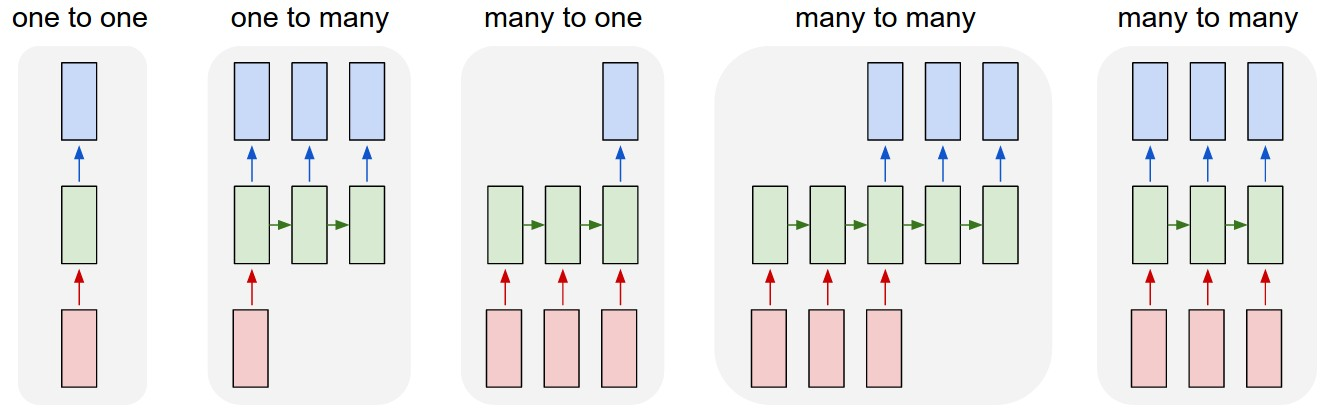
\includegraphics[scale=0.33]{images/inpoutp.jpeg}
    \caption{Types of RNN input to output mappings \citep{karpathy}}
\end{figure}

\noindent In each of these cases one column represents one time step of an RNN where the red, green and blue rectangles represent the input, the hidden state, and the output, respectively. The arrows indicate the flow of information within the model from which is clear that the hidden state evolves over time and propagates information about the sequence to the outputs.

The data being processed could be anything that contains a 'time' dimension such as text, audio, DNA sequences, or financial market data. Consequently, RNNs are a very popular choice when dealing with NLP\footnote{Natural Language Processing} problems most notable of which are language translation, text summarization, and part-of-speech tagging. The basline RNN model architecture in those cases is an attentional encoder-decoder architecture proposed by \cite{bahdanau} which added an attention mechanism to an already existing encoder-decoder architecture \citep{original-enc-dec}.

\begin{figure}[H]
    \centering
    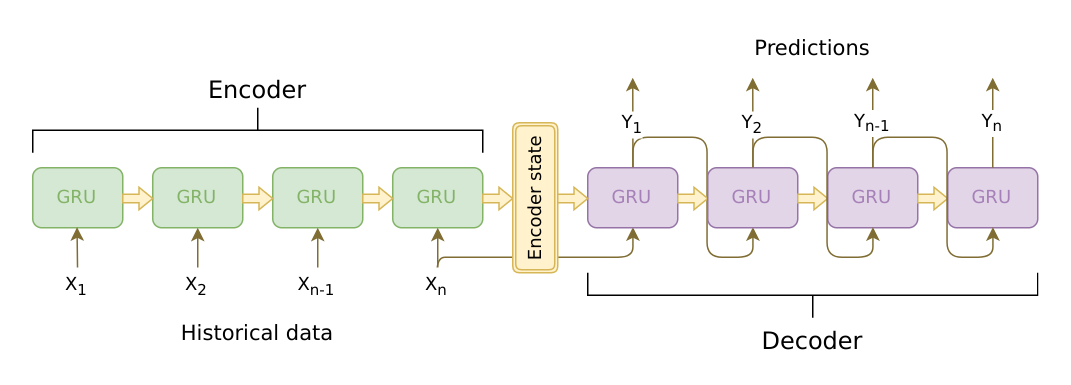
\includegraphics[scale=0.4]{images/enc_dec.png}
    \caption{RNN encoder-decoder architecture, source: \href{https://jeddy92.github.io/JEddy92.github.io/ts_seq2seq_intro/}{Joseph Eddy}}
\end{figure}

With everything said in mind, an RNN seems like an interesting candidate for experimenting with different tasks and measuring performance. In this paper, an attentional RNN encoder-decoder model is implemented and tasked with generating a title for an article given its abstract. This was chosen specifically because the task is comparable to an already well-studied problem of text summarization and because it is different in a way that articles don't necessarily have to summarize the article itself in an obvious way.

\section{Related work}

In recent years, when it comes to NLP related tasks, RNN models have been outperformed by transformer models \citep{transformers}. Most notable of which are Google's BERT \citep{bert} which works best on discriminative tasks, OpenAI's GPT-3 \citep{gpt3} designed for generative tasks, and Facebook's BART \citep{bart} which combines the concepts from the previous two. While they're very robust and seemingly able to perform any language specific task, such as the one this paper is trying to achieve, they are very large, can take relatively long time to fine-tune, and simply aren't always necessary for every task. That being said, RNNs are still being used either in conjunction with transformers or in standalone models where transformers aren't necessary or don't perform as well. In the case of title generation, while certainly able to perform the task, they might not be necessary.

Title generation is a task very similar to abstractive\footnote{As opposed to extractive, which extracts key sentences from the document instead of generating new ones.} text summarization already focused on by \cite{abstractive-text} where they use a model similar to the one used in this paper to scan an entire document with the goal of generating an abstractive summarization in the form of a few sentences. Their model is based on the aforementioned attentional RNN encoder-decoder model proposed by \cite{bahdanau} with additional upgrades. They implement a feature rich encoder which takes into account linguistic features of the word alongside the word itself, a switching generator-pointer mechanism which helps to deal with words not present in the dictionary, as well as a hierarchical attention mechanism which modifies the attention to work on both word and sentence level.

Additionally, there have been many proposed architectures and alternative approaches which improved upon the results achieved by Nallapati et al. One such proposal came from \cite{abs-improve} whose model borrowed concepts from variational auto-encoders introducing their generative latent structure to its architecture which improved results. Other approaches include those using convolutional neural networks \citep{cnn-abs} and generative adversarial networks \citep{gan}. An overview of these papers, as well as some others, can be read in a study by \cite{overview}.

Generally, most of these improvements exist because the task of generating an abstractive text summarization has to deal with a very large input size, whereas our model only has to deal with abstracts, which are much shorter. Because of this, our model resembles the one proposed by Bahdanau \citep{bahdanau}.
% which in this case is??

\section{Methodology}

\subsection{Dataset Description}

The entire dataset was acquired from \href{https://www.arxiv.org}{arXiv.org} using Python's \href{https://pypi.org/project/arxiv/}{arXiv API} querying the following keywords:
\begin{center}
\fbox{\parbox{\textwidth}{science, technology, biology, computer science, medicine, machine learning, equation, deep learning, distribution, learning, generation, model, image, graph, estimation, tree, molecule, quantum, genetic, computing, dna, engineering, data, study, advanced, astronomy, astrophysics, atom, beaker, biochemistry, chemistry, botany, cell, chemical, climate, control, electricity, element, energy, evolution, fossil, geology, geophysics, gravity, hypothesis, immunology, magnet, matter, meteorology, motion, organism, observe, phase, particle, physics, quantum mechanics, research, radiology, temperature, theory, tissue, variable, variational, volume, weather, zoology}}
\end{center}

\noindent Bias could exist in the keyword selection since they were chosen mostly arbitrarily and weren't given much thought. Nevertheless, $187538$ unique title-abstract pairs were acquired in this way. Some of the entries from the dataset are shown below, abstracts were shortened for brevity.

\begin{figure}[H]
    \centering
    \begin{tabular}{l|l}
        \toprule
            Title &                                           Abstract \\
        \hline
        \midrule
        The Science of al-Biruni & Al-Biruni (973-1048) was one of the greatest sc... \\
        Embracing Data Science & Statistics is running the risk of appearing irr... \\
        A New Task for the Philosophy of Science & This paper argues that philosophers of science ... \\
        Science and Philosophy: A Love-Hate Relationship & In this paper I review the problematic relation... \\
        Quantum Computer Systems for Scientific Discovery & The great promise of quantum computers comes wi... \\
        A note on two notions of compliance & We establish a relation between two models of c... \\
        \bottomrule
    \end{tabular}
    \caption{Example entries in the dataset}
    \label{fig:entries_data}
\end{figure}

Statistical analysis of the dataset concluded with the following results:

\begin{table}[H]
    \centering
    \begin{tabular}{l|l|l}
        \toprule
        \multicolumn{3}{c}{Word length} \\
        \hline
        & Titles & Abstracts \\
        \hline
        \midrule
        Min & 1 & 1\\
        Max & 47 & 619\\
        Median & 10 & 145\\
        Mean & 10.74488370356941 & 150.26933208203138\\
        Standard deviation & 4.100086118821517 & 64.23186043180522\\
        \bottomrule
    \end{tabular}
    \caption{Dataset statistics}
    \label{fig:word_len_stats}
\end{table}

\begin{figure}[H]
    \centering
    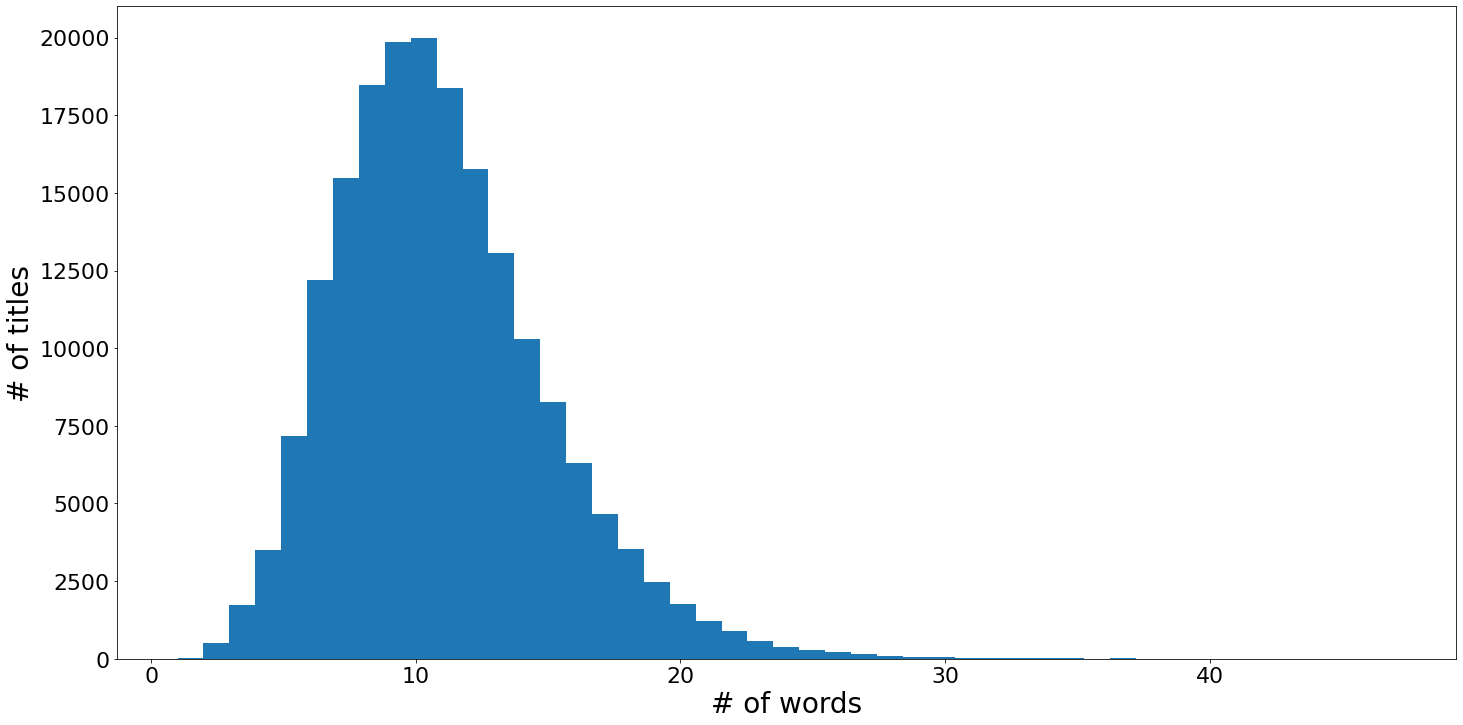
\includegraphics[scale=0.3]{images/titles_words_hist.png}
    \caption{Histogram showing the title word length distribution in the dataset}
\end{figure}

\begin{figure}[H]
    \centering
    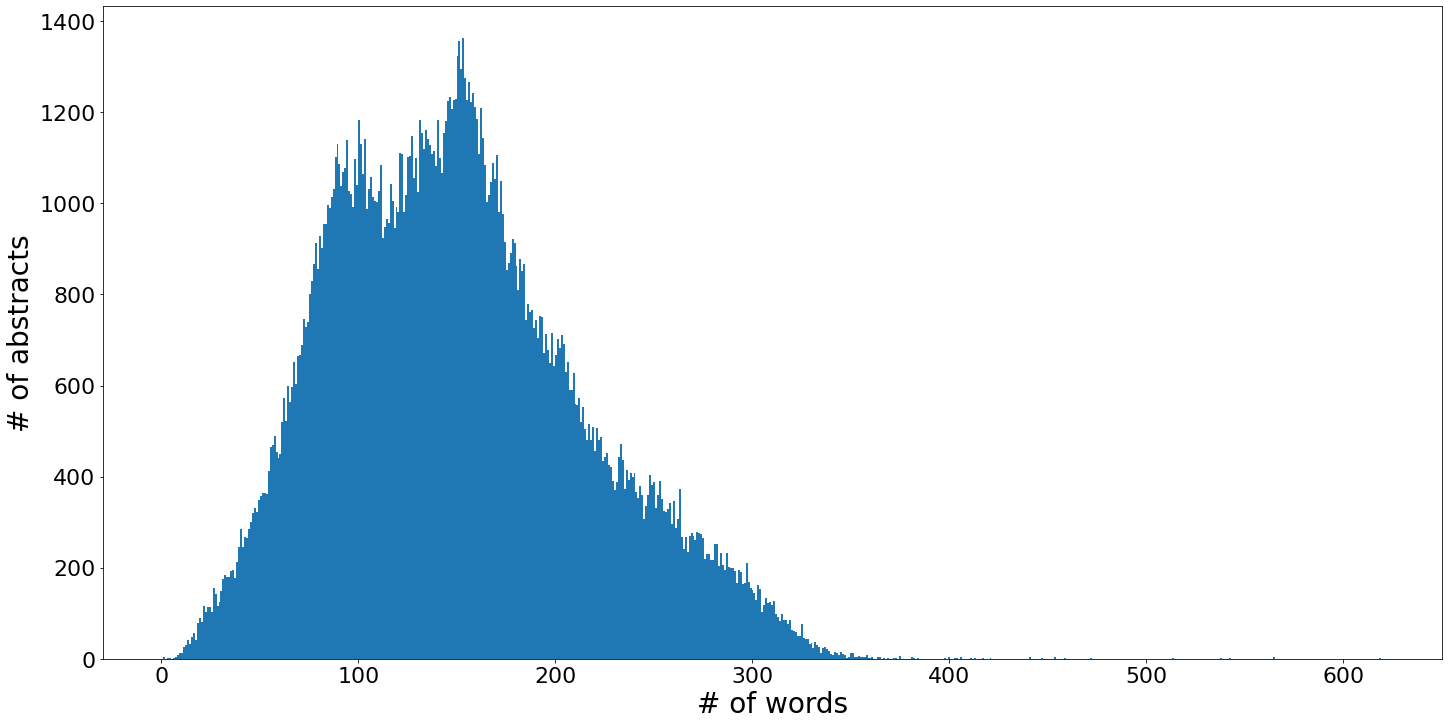
\includegraphics[scale=0.3]{images/abstracts_words_hist.png}
    \caption{Histogram showing the abstract word length distribution in the dataset}
\end{figure}




\subsection{Dataset Preprocessing}

All of the words in the dataset were lowercased and tokenized. In tasks such as sentiment analysis, removing stop words generally improves performance, but in tasks such as this one context is essential and stop words greatly contribute to it, therefore \textbf{no} stop words were removed. Additionally, dataset entries whose titles exceeded more than $24$ words were also removed prior to training because such entries would often cause out of memory issues. Alternatively, these issues could have been resolved by reducing the training batch size, but given that there are only $1036$ entries that have titles whose word count exceeds $24$, removing such entries seemed preferable to extending the time it takes to train the model. Dataset was then split into the traditional training, validation and test subsets in a ratio of $140000:23251:23251$.

The memory bottleneck of every sequence to sequence model is the size of its output dimension, in other words, its vocabulary. Because of this and because the model was trained on a GPU with only 4 GiB of memory, the vocabulary was constructed with words from the training subset only whose frequency is $10$ or higher. During training, if the word was not in the vocabulary it was replaced with the unknown token.

Lastly, a word embedding matrix was partially initialized using \href{https://www.kaggle.com/datasets/leadbest/googlenewsvectorsnegative300}{GoogleNews-vectors-negative300} dataset which maps words to 300 dimensional vectors. Every word that wasn't in the dataset was initialized randomly following the normal distribution $\mathcal{N}(0, 1)$. All of the values in the embedding matrix were set as trainable.

\subsection{Model Description}

The model follows the attentional encoder-decoder architecture proposed by \cite{bahdanau}, the only difference being the use of Luong's attention \citep{luong}. The main idea is to use the encoder to process an entire input sequence into a hidden state which the decoder then uses to generate a new sequence. The issue with this approach is that it's generally very difficult to encode all of the necessary information within the hidden state. This is why we need attention.

Besides updating the hidden state after each step, an RNN cell also generates an output. The idea behind attention is to somehow utilize the encoder cell outputs in the generation process. This is done for each time step in the decoder by calculating a context tensor based on the current hidden state, current decoder input and all of the encoder outputs. Attention is then defined as a normalized vector which denotes how important an encoder output is for the current time step, which when multiplied with the encoder outputs results in the context tensor.
\begin{equation}
    \textbf{c}_i = \textbf{a}_i \cdot \textnormal{enc\_out}
\end{equation}

This context tensor, along with the hidden state and an embedded input word, is then used as an input into the decoder's RNN cell to generate a new word. Luong expands on this and generalizes attention by adding an arbitrary scoring layer and using it on the context and the hidden state before using them as inputs to the cell, adding more flexibility. In this particular case, an arbitrary scoring layer was implemented by introducing additional parameters within the calculation and adding a \textit{tanh} activation function.

\begin{figure}[H]
    \centering
    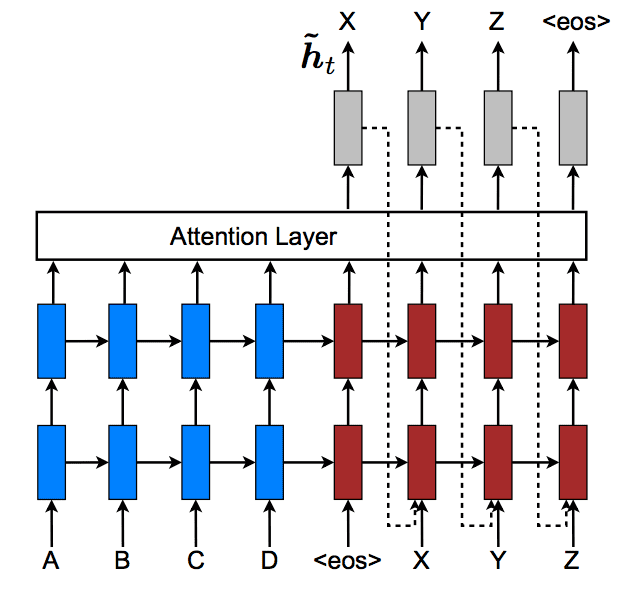
\includegraphics[scale=0.55]{images/attnencdec.png}
    \caption{Attentional RNN encoder-decoder architecture \citep{luong}}
\end{figure}

\begin{figure}[H]
    \centering
    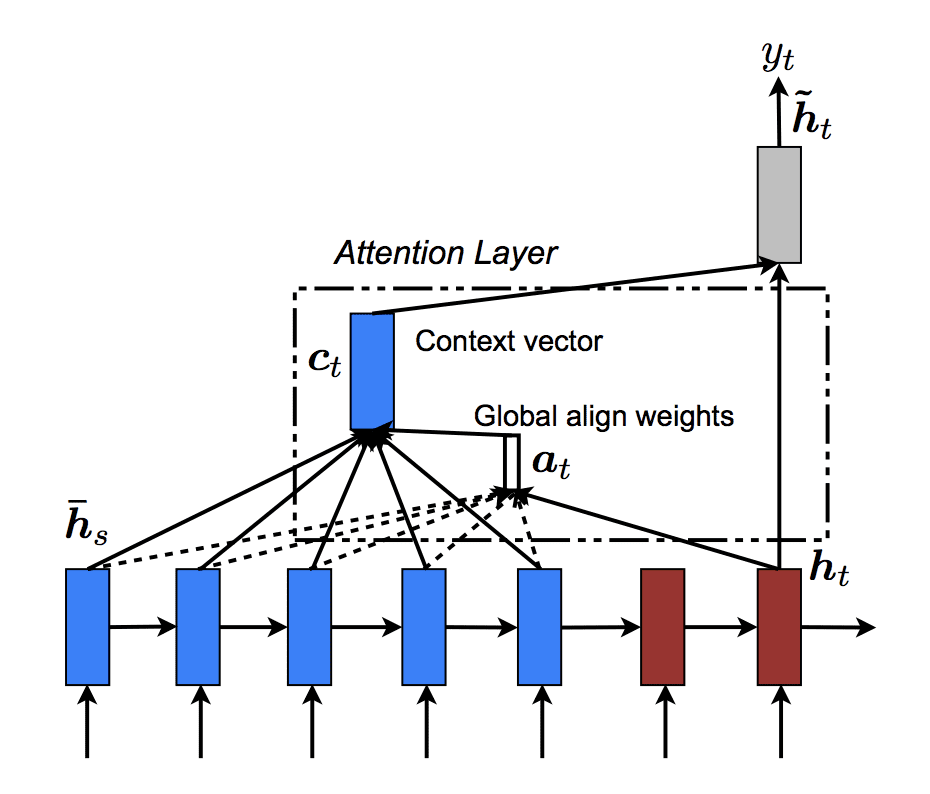
\includegraphics[scale=0.5]{images/attn_calc.png}
    \caption{Depiction of how attention is calculated \citep{luong}}
\end{figure}

The \textbf{encoder} itself consists of a bidirectional GRU cell \citep{gru} which takes a previous\footnote{In the first time step, the hidden state is initialized to zeros.} hidden state $h_{i-1}$ and an embedded input word tensor $x_i$ and outputs an updated hidden state $h_i$ and an output tensor $y_i$.
\begin{equation}
    \textnormal{GRU}_E(h_{i - 1}, x_i) = h_i\textnormal{, }y_i
\end{equation}
The embedded word tensor has a dimension of $300$, and because the cell is bidirectional, the output tensor and the hidden state are each composed of two $300$ dimensional tensors ($2 \times 300$), one for each direction. After processing an entire input sequence, the final hidden states are passed through a fully connected layer and transformed into a singular hidden state of size $300$, while the outputs are simply concatenated in a tensor of size $600$. The outputs of the encoder are then the final combined hidden state and the concatenated output tensors of the cell at each time step.
\begin{equation}
    \textnormal{Encoder}(x_{i...n}) = h_n\textnormal{, }y_{i...n}
\end{equation}

The \textbf{decoder} consists of an attention layer that calculates the context tensor $c_i$ and a unidirectional GRU cell whose inputs are the hidden state $h_{i-1}$ and the previously generated\footnote{At the start of generation, a start-of-sentence token is given as an input word.} input word $w_i$ concatenated with the context tensor, which together have a dimension size of $900$, meaning $300$ each. Outputs of the cell are the updated hidden state $h_i$ and the cell output tensor $y_i$, each of size $300$ as well.
\begin{equation}
    \textnormal{GRU}_D(h_{i - 1}, \textnormal{cat}(w_{i-1}, c_i)) = h_i\textnormal{, }y_i
\end{equation}
Lastly, the cell output tensor, context tensor, and the embedded input tensor are passed through a fully connected layer to produce a word predictions tensor $W_i$ which holds the probabilities for each word in the dictionary. This means that $W_i$ has a dimension size equal to the size of the dictionary which is $33278$.
\begin{equation}
    \textnormal{FC}(y_i, c_i, w_{i-1}) = W_i
\end{equation}
\begin{equation}
    \textnormal{Decoder}(h_{i - 1}, w_{i-1}, y_{i...n}) = W_i
\end{equation}

Since the predicted word is used in the next time step of the decoder, $W_i$ first needs to be converted to an index of the highest probability and then embedded using the embedding matrix.
\begin{equation}
    w_i = \textnormal{embedding\_matrix}[\textnormal{argmax}(W_i)]
\end{equation}

The model as described has 55M trainable parameters. While that describes most of the model, some of the details were omitted, such as the exact implementation of the attention layer and which activation functions were used. Luckily, all of that and more can be found on my \href{https://github.com/dominik-matic/nlp-seq2seq-title-generation}{github} page.



\subsection{Training the Model}

The model was trained with a batch size of $16$ across $15$ epochs. The initial learning rate was set to $1\cdot10^{-3}$ and was gradually lowered using an exponential LR scheduler with a gamma of $0.85$. 
\begin{figure}[H]
    \centering
    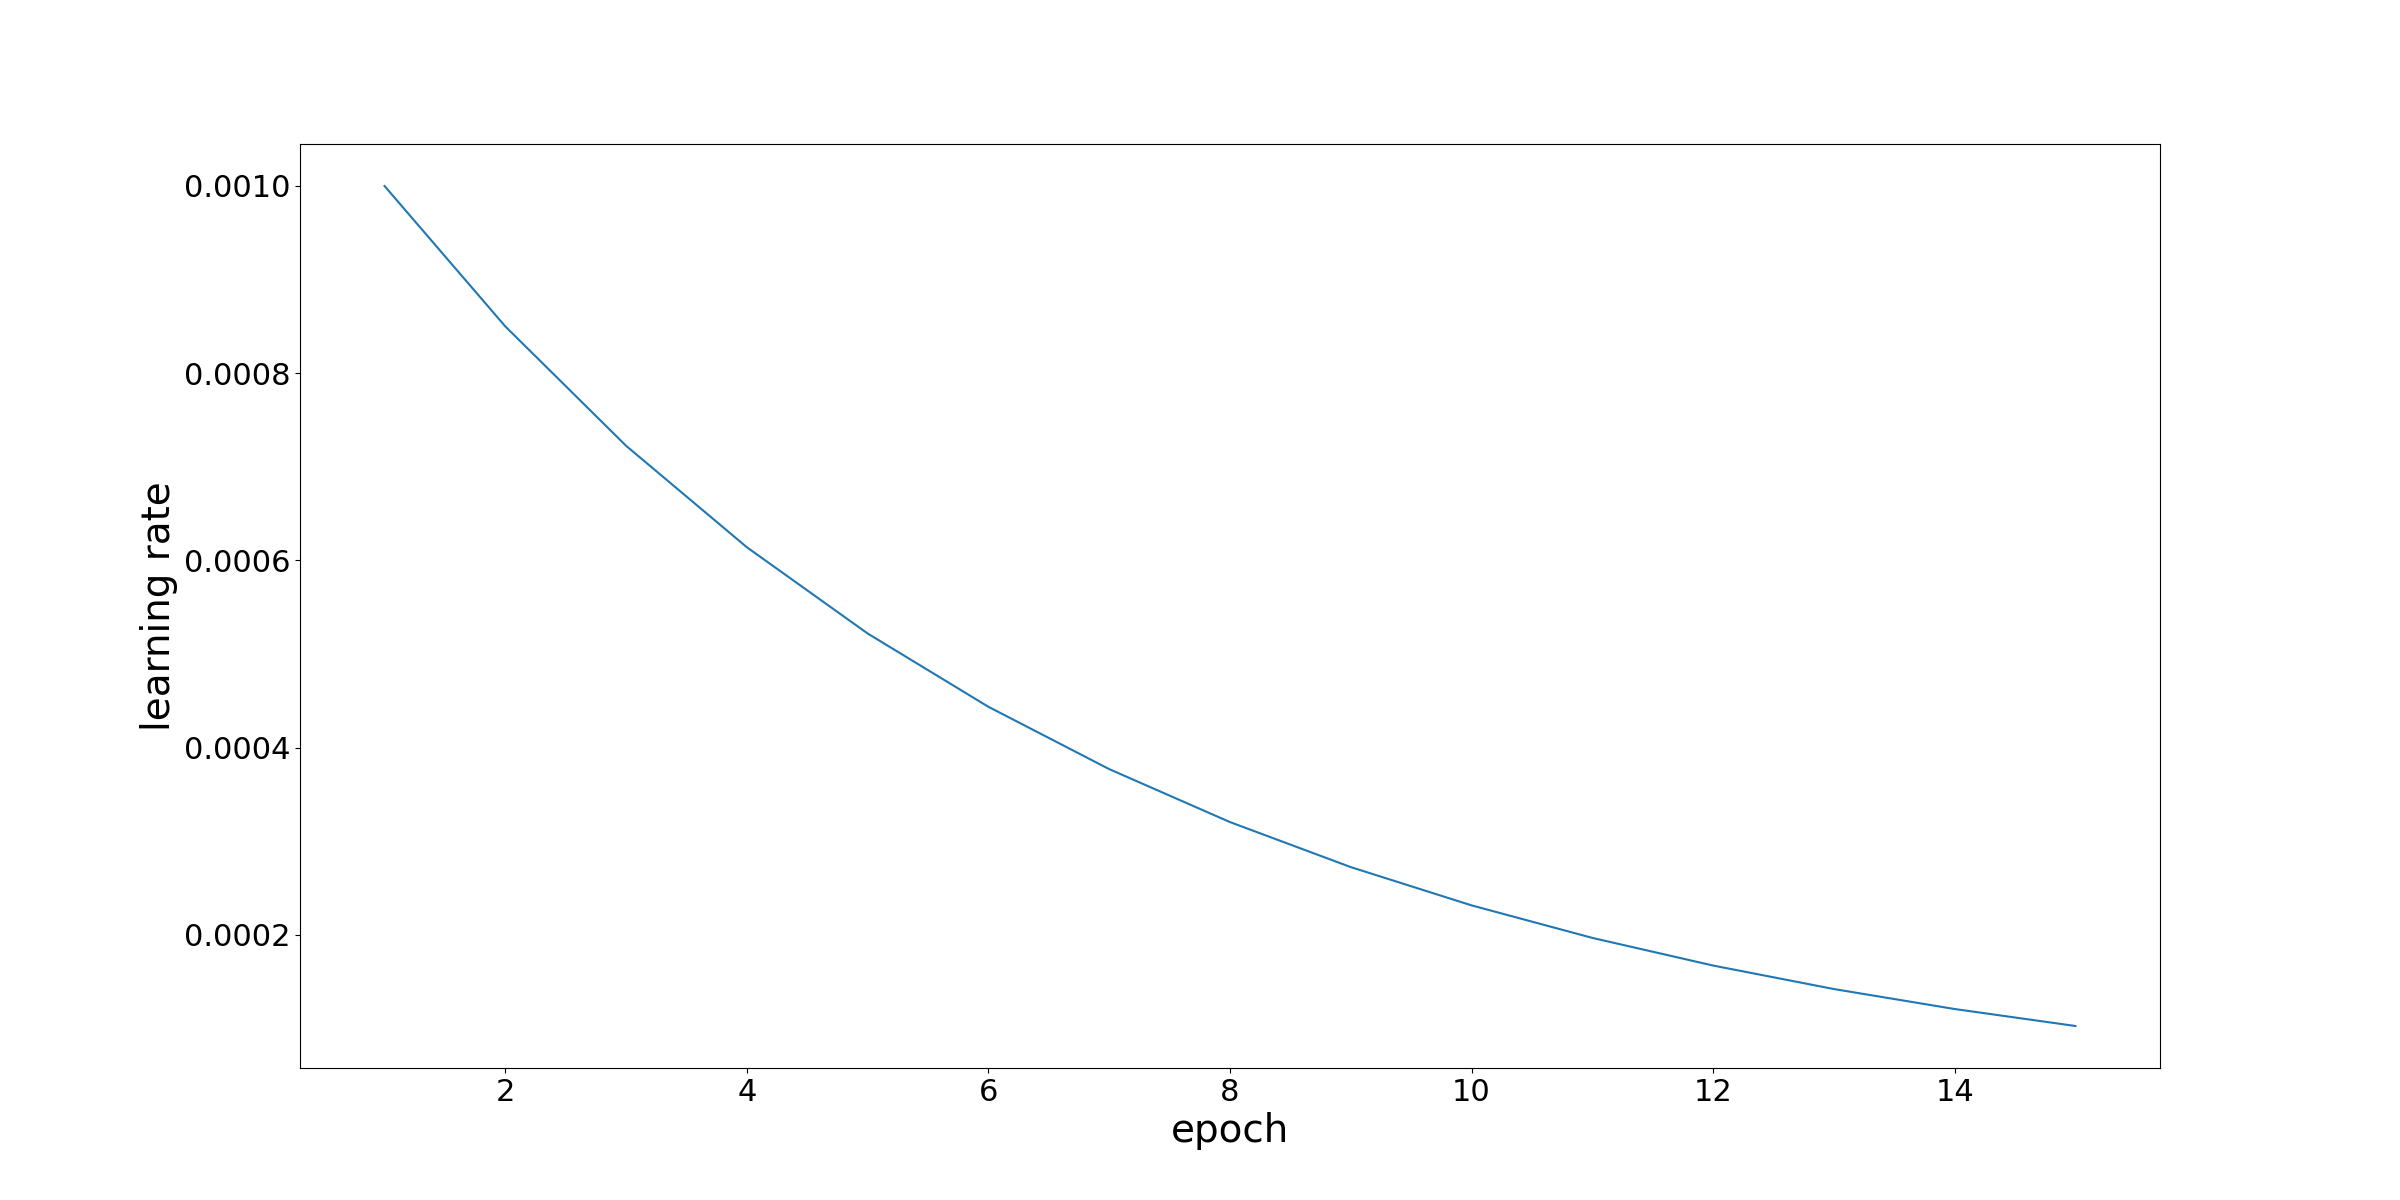
\includegraphics[scale=0.25]{images/lr_epochs.png}
    \caption{Learning rate through the epochs}
\end{figure}

During trainig, three key mechanisms were utilized: dropout, teacher forcing, and gradient clipping. Dropout layers were added as a form of regularization in both the encoder and the decoder acting on the embedded inputs; $x_i$ in the encoder and $w_i$ in the decoder. Both of the dropout layers were set to have a dropout probability of $0.5$. Teacher forcing is a method that improves learning by sometimes feeding the decoder a word it \textit{should} have generated, instead of the word it did generate. The rate of teacher forcing was set to $0.5$. Lastly, gradient clipping is a must when training recurrent models since they often have issues with exploding gradients. To avoid this, gradient clipping is applied by calculating the norm of all gradients and then clipping the gradients above a certain set value, in this case it was set to $0.5$.

Cross entropy was used as a loss function and its value was recorded every 20 batches:
\begin{figure}[H]
    \centering
    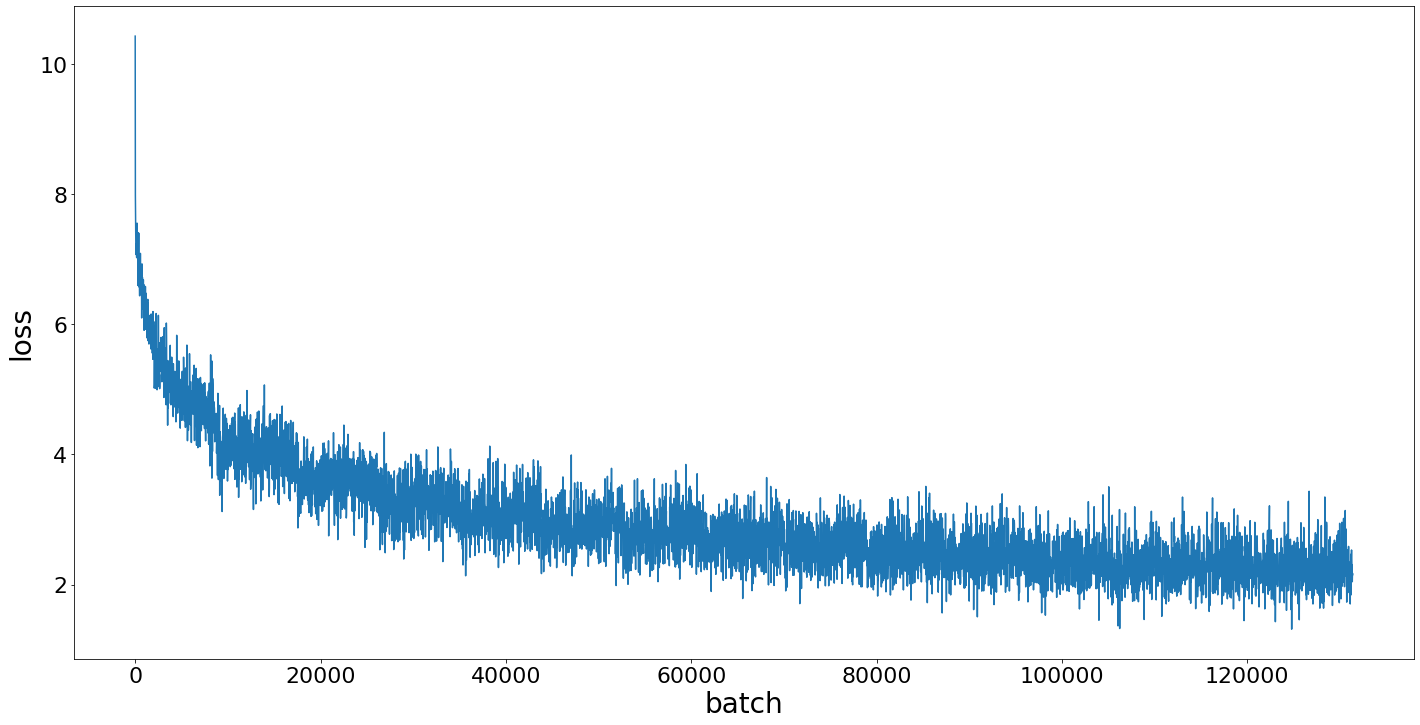
\includegraphics[scale=0.25]{images/train_loss.png}
    \caption{Loss during training}
\end{figure}

Model parameters were saved after each epoch so that early stopping could be used to detect  overfitting, that is to decide which version of parameters to use when evaluating on the testing set. While the average training loss was the lowest in epoch 15, being approximately $2.2475$, the average validation loss was lowest in epoch 14, amounting to $4.1270$. 
\begin{figure}[H]
    \centering
    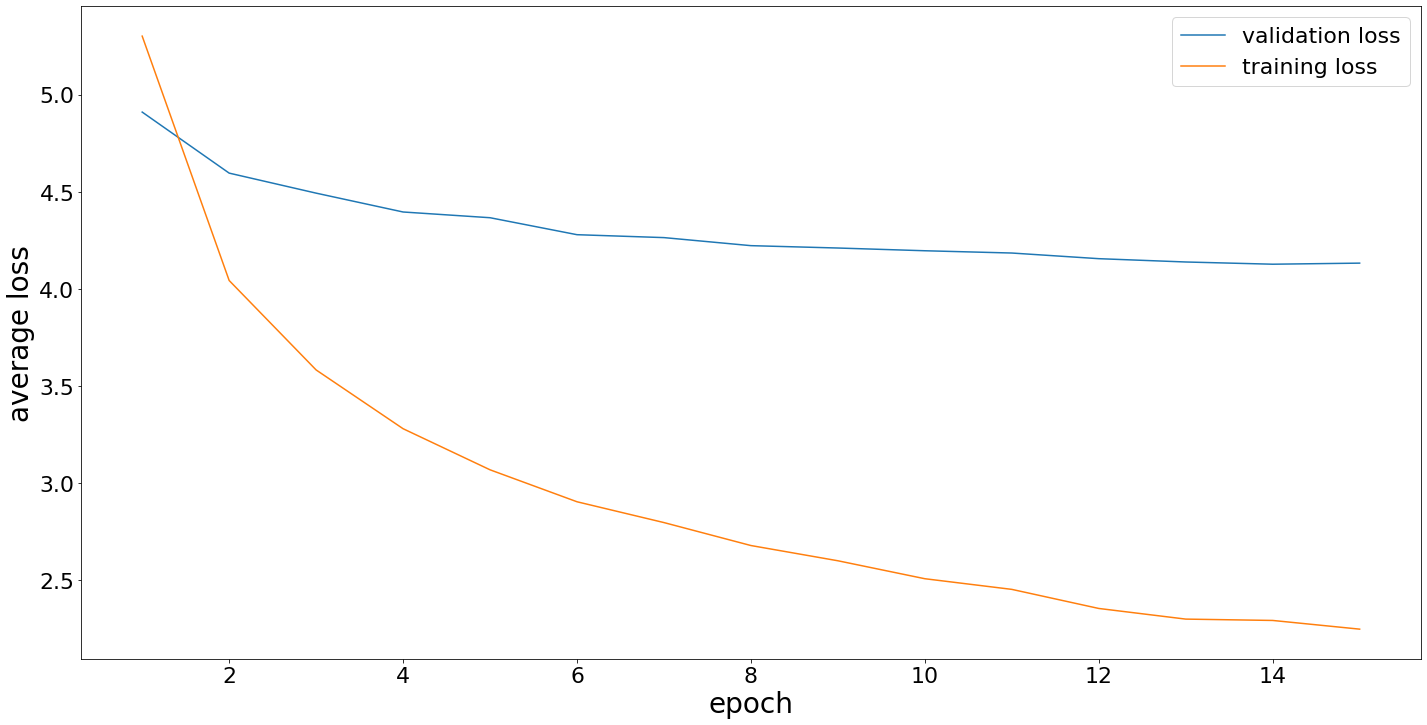
\includegraphics[scale=0.25]{images/valid_train_loss.png}
    \caption{Average validation and training loss across epochs}
\end{figure}
\noindent Evaluating the model from epoch 14 on the testing set resulted in the average loss of $4.1252$.


\section{Results}

To evaluate how well the model performs, we can utilize the ROUGE metric \citep{rouge} which was originally designed to evaluate the quality of text summarizations. It compares the generated output with reference outputs and counts the overlapping units such as unigrams (R1), bigrams (R2) or subsequences (RL). Using ROUGE to compare generated titles against actual titles from the validation and test set yields the following results:

\begin{table}[H]
    \centering
    \begin{tabular}{l|l|l|l}
        \toprule
        & R1 & R2 & RL \\
        \hline
        \midrule
        F-measure & 48.78 & 25.06 & 46.62\\
        Precision & 53.58 & 27.50 & 51.09\\
        Recall & 47.58 & 24.74 & 45.58\\
        \bottomrule
    \end{tabular}
    \caption{Evaluation of the model using the ROUGE metric}
    \label{fig:word_len_stats}
\end{table}

For comparison's sake, the following is the ROUGE table presented in the previously mentioned paper by \cite{abstractive-text} which focuses on abstractive text summarization. Of course, title generation and text summarization are different tasks, but it helps to build intuition of the metric.

\begin{table}[H]
    \centering
    \begin{tabular}{l|l|l|l}
        \toprule
        Model & Rouge-1 & Rouge-2 & Rouge-L \\
        \hline
        \midrule
        TOPIARY & 25.12 & 6.46 & 20.12\\
        ABS & 26.55 & 7.06 & 22.05\\
        ABS+ & 28.18 & 8.49 & 23.81\\
        RAS-Elman & \textbf{28.97} & 8.26 & 24.06\\
        words-lvt2k-1sent & 28.35 & \textbf{9.46} & 24.59\\
        words-lvt5k-1sent & 28.61 & 9.42 & \textbf{25.24}\\
        \bottomrule
    \end{tabular}
    \caption{ROUGE Recall table presented in \cite{abstractive-text}}
    \label{fig:word_len_stats}
\end{table}

When it comes to individual examples of generated titles, the quality can varies from excellent to not so much, where the average lies somewhere in between. Here are some examples, T/G meaning True/Generated:

\begin{center}
    \begin{longtable}{r|p{15cm}}
        \toprule
        T/G & Title  \\
        \hline
        \endhead
        \midrule
        T & testing the dark matter scenario for pev neutrinos observed in icecube \\
        G & testing the dark matter with icecube pev neutrinos\\
        \hline
        T & phase transition in loop quantum gravity \\
        G & phase transition in loop quantum gravity\\
        \hline
        T & simple alcohols with the lowest normal boiling point using topological indices \\
        G & simple alcohols of the lowest normal boiling point \\
        \hline
        T & a note on list coloring powers of graphs \\
        G & a note on the \textless UNK\textgreater  graphs\\
        \hline
        T & complete solution of a gauged tensor model \\
        G & complete analytic solution of the gauged gauged gauged gauged gauged gauged gauged gauged model\\
        \hline
        T & on various confidence intervals post model selection \\
        G & on confidence intervals in the <UNK> model\\
        \hline
        T & collective motion of oscillatory walkers \\
        G & collective motion of oscillatory walkers oscillatory walkers\\
        \hline
        T & outline of a generalization and a reinterpretation of quantum mechanics recovering objectivity \\
        G & outline of a quantum model for quantum mechanics\\
        \hline
        T & variational quantum circuit model for knowledge graphs embedding \\
        G & variational quantum circuit for knowledge graphs\\
        \hline
        T & robust information propagation through noisy neural circuits \\
        G & robust information of information in limited limited neural networks\\
        \hline
        T & computer simulations of single particles in external electric fields \\
        G & computer simulations of single particles in external electric fields\\
        \hline
        T & stability estimates for systems with small cross diffusion \\
        G & stability estimates for nonlinear diffusion problems with nonlinear diffusion terms\\
        \hline
        T & malicious web domain identification using online credibility and performance data by considering the class imbalance issue \\
        G & malicious web domain identification using deep learning\\
        \hline
        T & statistical tests for <UNK> pseudorandom number generator \\
        G & statistical tests of pseudo random number pseudo <UNK> numbers\\
        \hline
        T & electrical properties of chain microstructure magnetic emulsions in magnetic field \\
        G & electrical properties of chain microstructure magnetic emulsions\\
        \hline
        T & bringing quantum mechanics to life from schr\"{o}dinger s cat to schr\"{o}dinger s microbe \\
        G & bringing quantum cat and the microbe\\
        \hline
        T & astrophysical neutrinos flavored with beyond the standard model physics \\
        G & astrophysical neutrinos beyond astrophysical standard model\\
        \hline
        T & dark energy from the gravity vacuum \\
        G & dark energy in quantum gravity\\
        \hline
        T & quantum computation toolbox for decoherence free qubits using multi band alkali atoms \\
        G & quantum engineering of qubits with ultracold atoms\\
        \hline
        T & probing a gravitational cat state \\
        G & probing the cat state in a gravitational cat state\\
        \hline
        T & evolutionary techniques in lattice sieving algorithms \\
        G & evolutionary lattice lattice lattice lattice lattice lattice\\
        \hline
        T & quantum dynamics of the early universe \\
        G & quantum corrections to the early universe\\
        \hline
        T & non stationary spectral kernels \\
        G & non stationary spectral kernels for non stationary kernel process\\
        \hline
        T & toward automatic verification of quantum programs \\
        G & toward automatic verification of quantum programs\\
        \hline
        T & fifty years of energy extraction from rotating black hole revisiting magnetic penrose process \\
        G & fifty years of a penrose process\\
        \hline
        T & transition probability estimates for long range random walks \\
        G & transition and discrete step rates for discrete time spaces\\
        \hline
        T & qubit entanglement across epsilon near zero media \\
        G & qubit materials near near materials materials materials \\
        \hline
        T & equations defining probability tree models \\
        G & models of the trees in tree tree\\
        \hline
        T & graphene plasmonics \\
        G & graphene plasmonics graphene plasmonics\\
        \hline
        T & a refined analysis on the x 3872 resonance \\
        G & a study d bar d j d j d j d j d j d d d j d\\
        \hline
        T & asymptotic equivalence of quantum stochastic models \\
        G & asymptotic convergence of quantum stochastic models\\
        \hline
        T & energy level statistics in strongly disordered systems with power law hopping \\
        G & energy level statistics statistics of disordered disordered systems\\
        \hline
        T & on the various aspects of electromagnetic potentials in spacetimes with symmetries \\
        G & on the killing killing killing killing killing killing killing killing killing killing killing killing killing vector fields\\
        \hline
        \bottomrule
        \caption{Examples of generated sentences}
    \end{longtable}
\end{center}

It is also clear that model suffers from neural text degeneration meaning it repeats some words or phrases multiple times. It is an interesting phenomenon and there are proposed solutions to combat it \citep{degen}. All of the generated titles, alongside the model itself and the dataset can be found on my \href{https://github.com/dominik-matic/nlp-seq2seq-title-generation}{github} page.

\section{Discussion}

There are many factors which influence how any given model will perform. In this particular case, there are several ways in which the model could be improved. One such way would be a better sanitation and tokenization of the dataset. For example, numbers and similar symbols could be removed from the vocabulary and a previously mentioned switching generator-pointer mechanism \citep{abstractive-text} could be implemented to deal with words not present in the dictionary. Of course, a better dataset could be used as well, one less scientific, perhaps.

One potentially simple improvement would be to implement a separate embedding matrix for the decoder which would increase the number of trainable parameters significantly, but as GPT-3 has shown, when it comes to language models, bigger is better.

As mentioned, the model suffers from a case of neural text degeneration. An interesting experiment would be to implement Nucleus Sampling proposed by \cite{degen} to see if the problem persists. 

It is also possible a slightly different model configuration could have yielded better results since the single greatest obstacle in the way of achieving such results in the scope of this paper was certainly the hardware available for training. 
The model was implemented to be highly customizable and as such it could have been easily modified and tested with many different configurations, if the hardware were to allow it. Which sadly wasn't the case here. With more and better GPUs, batch size could be increased, training time reduced resulting in an easier time of fine-tuning the hyperparameters for this specific task. If none of that yields satisfactory results, the next logical step would be to move onto the transformer architecture.


\bibliographystyle{johd}
\bibliography{bib}

%\section*{Supplementary Files (optional)}
%Any supplementary/additional files that should link to the main publication must be listed, with a corresponding number, title and option description. Ideally the supplementary files are also cited in the main text.
%Note: supplementary files will not be typeset so they must be provided in their final form. They will be assigned a DOI and linked to from the publication.

\end{document}